%%%%%%%%%%%%%%%%%%%%%%%%%%%%%%%%%%%%%%%%%%%%%%%%%%%%%%%%%%%%%%%%%%%%%%%%%%%%%%%%
%2345678901234567890123456789012345678901234567890123456789012345678901234567890
%        1         2         3         4         5         6         7         8

\documentclass[letterpaper, 10 pt, conference]{ieeeconf}  % Comment this line out if you need a4paper

%\documentclass[a4paper, 10pt, conference]{ieeeconf}      % Use this line for a4 paper
\usepackage{times}
\usepackage[dvipsnames,table]{xcolor}
\usepackage{multicol}
\usepackage[bookmarks=true]{hyperref}
\usepackage{graphicx}
\usepackage{algorithm}
\usepackage{amsmath}
\usepackage[normalem]{ulem}
\usepackage{subcaption}
\usepackage{amssymb}
\usepackage{booktabs} % For professional looking tables (\toprule, \midrule)
\usepackage{multirow} % To combine rows for the Task Suites
\usepackage{tcolorbox}
\usepackage{siunitx}

\usepackage{booktabs}
\usepackage{caption}
%\usepackage{enumitem}

\usepackage[normalem]{ulem}

% first-column class colors
\definecolor{clsGeneralist}{RGB}{229,245,224} % light green
\definecolor{clsSpecialist}{RGB}{253,233,232} % light pink/red
\definecolor{clsOurs}{RGB}{232,240,255}       % light blue
\definecolor{clsPropGen}{RGB}{236,231,255}    % light  purple
\definecolor{bestCell}{RGB}{255,244,204}      % light yellow (best model)

% caption background (optional)
\definecolor{capbg}{gray}{0.93}
\DeclareCaptionFormat{colorbox}{
  \colorbox{capbg}{\parbox{\dimexpr\linewidth-2\fboxsep\relax}{#1#2#3}}
}
\captionsetup[table]{format=colorbox,labelfont=bf}

% tiny legend swatch
\newcommand{\swatch}[1]{\begingroup\setlength{\fboxsep}{1.2pt}\colorbox{#1}{\strut\hspace{0.9em}}\endgroup}

% Pick colors that match the highlights you’ll add in the figure
\definecolor{envCol}{RGB}{255,236,214}    % environment (orange-ish)
\definecolor{agentCol}{RGB}{232,240,255}  % agentic layer (blue-ish)
\definecolor{compCol}{RGB}{229,245,224}   % composition (green-ish)
\definecolor{metricCol}{RGB}{236,231,255} % metric kernel (purple-ish)
\definecolor{spatialCol}{RGB}{253,233,232}% spatial kernel (pink-ish)


\newcommand{\cA}[1]{\textcolor{envCol}{#1}}
\newcommand{\cB}[1]{\textcolor{agentCol}{#1}}
\newcommand{\cC}[1]{\textcolor{compCol}{#1}}

    
\newif\ifcomments
\commentstrue   % show comments
%\commentsfalse % hide comments

% The clean build mode defines \SUBMISSION, which force-hides every co-author
% note. Use the build script when notes must be hidden so they cannot leak.
\ifdefined\SUBMISSION\commentsfalse\fi

% Revision markup: \rev{...} wraps changed text.
% Set \revhlfalse when revisions should typeset as ordinary black text.
\newif\ifrevhl
\revhlfalse      % revisions typeset plain
%\revhltrue     % revisions highlighted for co-authors
\newcommand{\rev}[1]{\ifrevhl\textcolor{BrickRed}{#1}\else#1\fi}

% \newcommand{\opnote}[1]{\textcolor{blue}{#1}}
\newcommand{\opnote}[1]{\ifcomments\textcolor{blue}{#1}\fi}
\newcommand{\ngnote}[1]{\ifcomments\textcolor{olive}{#1}\fi}
\newcommand{\tn}[1]{\ifcomments\textcolor{teal}{#1}\fi}
\newcommand{\ljnote}[1]{\ifcomments\textcolor{cyan}{#1}\fi}
\newcommand{\spnote}[1]{\ifcomments\textcolor{green}{#1}\fi}
\IEEEoverridecommandlockouts                              % This command is only needed if 
                                                          % you want to use the \thanks command

\overrideIEEEmargins                                      % Needed to meet printer requirements.

%In case you encounter the following error:
%Error 1010 The PDF file may be corrupt (unable to open PDF file) OR
%Error 1000 An error occurred while parsing a contents stream. Unable to analyze the PDF file.
%This is a known problem with pdfLaTeX conversion filter. The file cannot be opened with acrobat reader
%Please use one of the alternatives below to circumvent this error by uncommenting one or the other
%\pdfobjcompresslevel=0
%\pdfminorversion=4

% See the \addtolength command later in the file to balance the column lengths
% on the last page of the document

% The following packages can be found on http:\\www.ctan.org
%\usepackage{graphics} % for pdf, bitmapped graphics files
%\usepackage{epsfig} % for postscript graphics files
%\usepackage{mathptmx} % assumes new font selection scheme installed
%\usepackage{times} % assumes new font selection scheme installed
%\usepackage{amsmath} % assumes amsmath package installed
%\usepackage{amssymb}  % assumes amsmath package installed

\title{\LARGE \bf
Meanings and Measurements: Multi-Agent Probabilistic Grounding for Vision-Language Navigation
}

\author{
\begin{tabular}{c}
Swagat Padhan$^{*,1}$, Lakshya Jain$^{*,1}$, Bhavya Minesh Shah$^{1}$, Omkar Patil$^{1}$, Thao Nguyen$^{2}$, Nakul Gopalan$^{1}$ \\[4pt]
$^{1}$Arizona State University \qquad $^{2}$Haverford College \\[2pt]
{\footnotesize \texttt{\{spadhan, ljain6, bshah43, opatil3, ngopalan\}@asu.edu, tnguyen3@haverford.edu}}
\end{tabular}
}



\begin{document}



\maketitle
\begin{figure}[b]
\vspace{-10pt}
\begin{tcolorbox}[
  colback=white,
  colframe=black,
  boxrule=0.3pt,
  arc=0pt,
  left=4pt, right=4pt, top=3pt, bottom=3pt,
  fontupper=\footnotesize
]
$^{*}$Equal contribution. This work was partly funded by TSMC and Arizona State University.
\end{tcolorbox}
\end{figure}
\thispagestyle{empty}
\pagestyle{empty}


%%%%%%%%%%%%%%%%%%%%%%%%%%%%%%%%%%%%%%%%%%%%%%%%%%%%%%%%%%%%%%%%%%%%%%%%%%%%%%%%
\begin{abstract}

%\opnote{I have added a lot of comments here- once you are done addressing a specific comment, 'comment' it out and don't delete it completely so that I can keep a track.}
\rev{Robots collaborating with humans must convert natural language goals into actionable, physically grounded decisions. Executing ``go two meters to the right of the fridge'' requires simultaneously resolving a semantic referent, interpreting a spatial predicate in a geometrically consistent frame, and enforcing an exact metric offset in $3$D space. We show empirically that existing VLM-based systems struggle with this joint requirement: scene-graph EQA approaches commit to a single target without metric enforcement, while single-image spatial specialists produce no actionable allocentric goals. To address this, we propose MAPG (Multi-Agent Probabilistic Grounding), a framework that treats metric-semantic goal grounding as compositional inference over $3$D space. MAPG decomposes a query into structured clauses, resolves referents via multi-view evidence accumulation against an online $3$D scene graph, and instantiates three analytic kernels per clause (semantic, metric, and directional) whose parameters are predicted by specialist VLMs. Kernels compose via a Product of Experts (log-space addition) into a continuous goal distribution $P(x)$ over free navigable space, directly consumable by a motion planner.} 
% \opnote{don't name the benchmark here, and what does it represent? Are you trying to say that your method leads to good performance even when metric component is absent from the query? The state it that way.} %\opnote{describe the baselines- like EQA baselines}
We introduce MAPG-Bench ($98$ queries, $41$ HM$3$D scenes), the first benchmark targeting metric-semantic goal grounding, and evaluate on existing embodied QA benchmarks to show competitive performance even when metric constraints are absent. In a completed end-to-end MAPG-Bench run, MAPG succeeds on $79$ of $98$ queries ($80.6\%$) and finds the anchor on $80$ ($81.6\%$). Separate component evaluation reduces object-to-world grounding error from $5.82\,\mathrm{m}$ to $0.07\,\mathrm{m}$ ($98.8\%$). %\opnote{by how much}
A real-world robot demonstration illustrates the approach outside simulation when a structured scene representation is available.
\end{abstract}


%%%%%%%%%%%%%%%%%%%%%%%%%%%%%%%%%%%%%%%%%%%%%%%%%%%%%%%%%%%%%%%%%%%%%%%%%%%%%%%%
\section{Introduction}
%\ngnote{The whole intro is a four part structure - what is the problem domain? What work exists and how does it fail? What is your novelty and why? What are your results? This intro does not follow that it meanders and presents opinions and approaches all over the place. Technical writing has to be crisp and tight with identifiable structure and narrative.}


Robots that collaborate with humans must be able to convert natural language goals into actionable, grounded decisions. People often mix metric and semantic specifications %\opnote{often mix metric and semantic- cut all the time}
- from ``being five minutes late'' to ``taking a left after about a mile on the highway.'' 
We refer to these as metric-semantic queries. The semantics relate to the attributes of an object or concept and spatial relationships such as left, right, front, behind; whereas the metric part of the query relates to measurable quantities such as distances, time and scale.
\begin{figure}
    \centering
    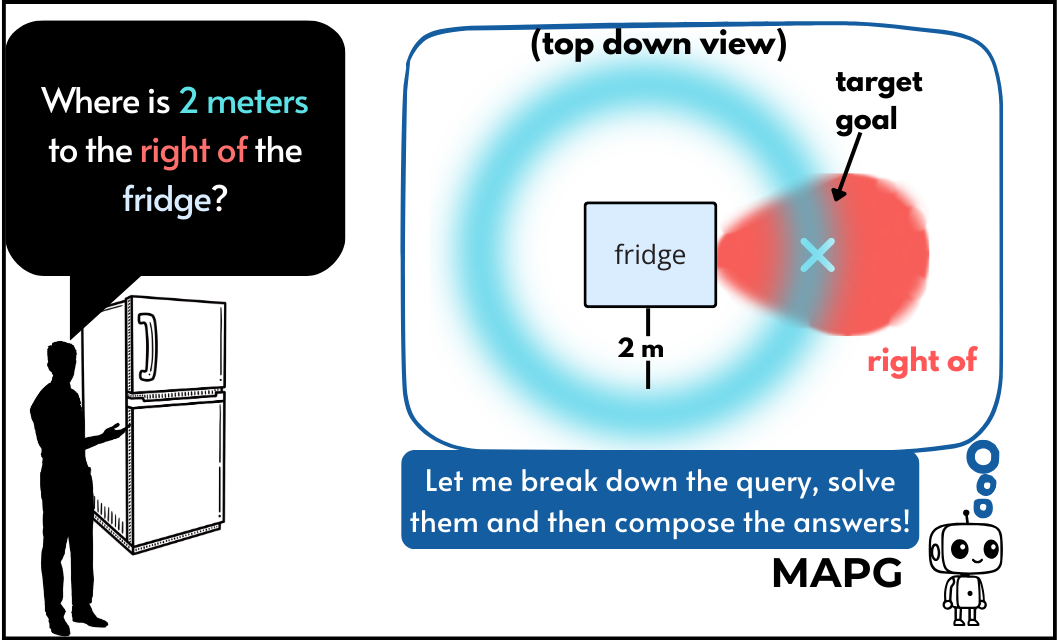
\includegraphics[width=1\linewidth]{figures/introfigure-rework.png}
    \caption{When a human specifies an open world metric-semantic query, referring to a location in the world, MAPG decomposes the query into subparts as learned probability distributions and composes them for grounding.
    }
    \label{fig:overview}
\end{figure}
Grounding these metric-semantic queries in a map requires jointly reasoning over referent semantics, spatial predicates, and metric scale, where the intended goal is a continuous region anchored to a grounded object pose.
%\ngnote{make this para tighter. I took a pass but it might have some facts missing. Also there is an argument to be made about single models needing more data when compared to using existing models compositionally.} \opnote{yes, read and use language from here: https://arxiv.org/abs/2402.01103v3.}

Instruction following is a central subfield of grounded language learning in robotics \cite{tellexlanguagesurvey}. Most existing systems ground language to actions or goals, which can be objects in a scene \cite{dai2024thinkactaskopenworld}. %\tn{https://arxiv.org/pdf/2310.07968, https://openreview.net/pdf?id=nNsZxc2cmO}. 
Several grounded language systems emphasized structured decomposition and probabilistic inference to connect linguistic constituents to world entities~\cite{tellex2011symbolgrounding}  while modern navigation and embodied question answering (QA) systems increasingly rely on large vision-language models (VLMs) and large language models (LLMs) to reason over observations and internal scene representations such as $3$D semantic scene graphs \cite{graphEQA, rana2023sayplan}. %\ngnote{whole line of work from cynthia matuszek and hadas kresgazit going from language to goals as well}
These approaches treat goal grounding as a single-step decision: given the current observation (and sometimes an internal map), the model is prompted to output either a discrete action or a single target hypothesis \cite{vsiBench,frameOfReferenceAmbiguity}.  However, such designs can be fragile for metric-semantic instructions whose correctness depends on precise geometry and a consistent frame of reference while navigating to discover the goal.
Furthermore, language grounding is bidirectional: the agent must convert egocentric observations into allocentric positions on the map, then convert an allocentric goal back into egocentric coordinates for execution, which compounds errors from each step.
% Since the system typically commits early to one target, recovery often reduces to heuristic retries rather than principled re-grounding in a persistent $3$D representation \cite{vsiBench,frameOfReferenceAmbiguity}.
% In embodied navigation, an agent typically receives egocentric sensory inputs over time and builds an allocentric spatial memory that supports planning.
% $3$D scene graphs are one such representation of the environment: they store object nodes with estimated poses and geometry, and support querying the environment in an object-centric and spatially structured way and it helps connect language to persistent world state, but metric-semantic goal grounding remains challenging under viewpoint changes, partial observability, and ambiguous frames of reference \cite{vsiBench,frameOfReferenceAmbiguity}.

% Existing embodied systems still struggle with metric-semantic goal grounding: general-purpose LLMs are unreliable for fine-grained metric spatial reasoning, and even scene-graph-based approaches often reduce goals to discrete targets rather than continuous spatial intent \cite{graphEQA}. These trends suggest a missing piece in the reasoning stack: a representation that is grounded for control, flexible to represent and update uncertainty, and compositional to support complex spatial instructions. We address this gap with Multi-Agent Probabilistic Grounding (MAPG), an agentic framework that produces planner-ready goal distributions for metric-semantic spatial instructions and add a probabilistic goal interface between foundation-model grounding signals and navigation affordances, representing the intended goal as a robust continuous distribution \(P(x)\) over $3$D space rather than as a single discrete target.

We propose MAPG (Multi-Agent Probabilistic Grounding), an agentic framework that queries different VLM Agents to produce probabilistic distributions and composes them into the goal. Given an instruction, MAPG decomposes it into structured clauses, resolves referents against an online $3$D scene graph and the current egocentric view, and instantiates analytic kernels for semantic, metric, and spatial constraints.
These kernels are then composed to produce a final goal density that better represents the spatial intention, which a planner can then query to generate executable waypoints.
Fig. \ref{fig:overview} shows an example of this approach.
%\opnote{also claim potentially better performance due to the fact that we can use expert models that are better at different aspects such as spatial reasoning.}
% \tn{cut: We instantiate this approach in a multi-agent architecture, that builds on the strengths of online $3$D scene graphs, composition and agentic frameworks.
% MAPG separates referent grounding from spatial inference: a Grounding Agent matches linguistic anchors (e.g., \emph{fridge}) to object instances in the scene graph using egocentric evidence, and a Spatial Agent outputs the parameters of the continuous probability field anchored at the resolved referent, which is then analytically composed into the final goal distribution.
% The planner then queries this goal distribution to propose candidate waypoints and selects a navigation action.}
%\opnote{talk more about the different agents you instantiate in the scene, what they return at a high level (parameters of a distribution) and how you compose them at a high level.}\ljnote{subsection 1 in method, could be moved here.} \tn{I only want a sentence, something like: We pre-specify the shape of the kernels and use different models to predict the kernel parameters based on...} 
% We evaluate this framework in Habitat simulation using HM$3$D scenes \cite{ramakrishnan2021habitatmatterport$3$Ddatasethm$3$D}, with a curated set of annotated metric-spatial queries that target object-to-world relationships in cluttered indoor environments. 
% We release this dataset and evaluation protocol to support reproducible comparison for metric-semantic goal grounding, and report results against VLM-based baselines and scene-graph-driven planners. 

Our main contributions are as follows: %\opnote{be more emphatic- and not dry in your contributions}:
\begin{itemize}
    \item \textbf{A multi-agent probabilistic $3$D spatial reasoning framework for goal grounding} that couples online $3$D scene graphs with analytically defined continuous spatial kernels to produce planner-ready goal distributions for metric-semantic instructions.
    \item \textbf{A first-of-its-kind HM$3$D~\cite{ramakrishnan2021habitatmatterport3ddatasethm3d} goal grounding benchmark for metric-semantic queries}, including an open-source dataset and evaluation protocol spanning $41$ unique indoor scenes and $98$ annotated metric-semantic queries designed for object-to-world goal grounding in realistic indoor layouts.
    \item \textbf{Empirical findings and ablations}: In a completed $98$-query end-to-end evaluation, MAPG succeeds on $79$ queries ($80.6\%$) and finds the anchor on $80$ ($81.6\%$). We additionally report predicate-level and target-distance breakdowns and provide a failure taxonomy for reproducible comparison.
\end{itemize}
Our webpage includes videos, benchmark examples, and extensive results: \opnote{website is not working} \href{https://sites.google.com/view/mapg-web/home}{sites.google.com/view/mapg-web/home}.
% full-width figure right after contributions
% \clearpage % optional: forces the page break here (use ONLY if you want to guarantee the break)
\begin{figure*}[t]
    \centering
    \vspace{1mm}
    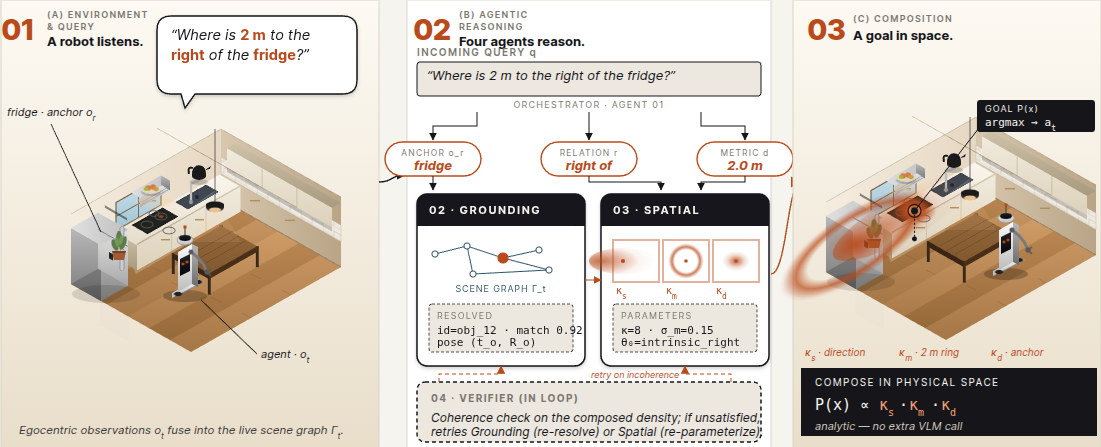
\includegraphics[width=0.99\linewidth]{figures/figure_2_new.png}
    \caption{\textbf{MAPG overview.}
    (a)~The robot observes a $3$D environment and receives a natural-language spatial query $q$.
    (b)~\emph{Agentic spatial reasoning layer}: the Orchestrator decomposes $q$ into anchor, relation, and metric tokens $\langle o_r, r, d\rangle$; the Grounding Agent resolves $o_r$ against the $3$D scene graph $\Gamma_t$ using multi-view evidence; the Spatial Agent emits parameters for the directional, metric, and anchor-density kernels. The Verifier closes a retry loop on incoherent compositions.
    (c)~\emph{Composition layer}: MAPG composes the analytic kernels in physical space to produce a continuous target-location PDF $P(x)$, planner-ready as a navigation or object-selection goal. \opnote{too much empty space}
    % \opnote{You don't talk about the logical agent in your methods section. The methods section and these diagrams need to present a consistent picture, and that is very important.}
    }
    \label{fig:method-overview}
\end{figure*}

\section{Background and Related Work}
Our work lies at the intersection of embodied vision-language navigation, structured $3$D spatial memory, spatial reasoning with multimodal foundation models, and probabilistic grounding. We review the most relevant directions and highlight the gaps our method addresses. %\opnote{like you said earlier, this section is too big right now. We should condense it to a page max. The way you do it like you hinted last time is to make a general/common statement followed by multiple citations, and not talk about each paper/work individually. your job in this, ironically, is not to educate but to complain about related works and argue conceptually that you are better/similar/different.}

%\tn{If you can reduce each subsection to a paragraph then you don't even need the subsections} 
\noindent{\textbf{{Embodied Question Answering and Vision-Language Navigation:}}}
Embodied Question Answering (EQA) and Vision-and-Language Navigation (VLN) both require an agent to ground language into actions over long horizons under partial observability, using only egocentric observations~\cite{das2018embodiedqa}.
Many embodied systems still commit to a single action or discrete target at each step, so early grounding errors compound and can derail the entire trajectory \cite{cohen2024surveyroboticlanguagegrounding,ahn2022saycan, dai2024thinkactaskopenworld}.
Some prior VLN-based works explicitly identify this issue and introduce backtracking and progress-based recovery to mitigate trajectory drift under greedy decisions~\cite{ma2019regretful}.
Conceptually, our approach addresses the same failure mode by shifting goal grounding to producing a planner-ready goal representation in a generated map rather than a one-shot action choice.
% , so that planning and execution can be driven by a geometric target distribution rather than by a one-shot action choice.
% \opnote{tie it back to your project. How does your work connect to long horizon planning?}
%\tn{cut: Our setting matches this regime, but focuses on a failure point that becomes dominant in long-horizon behavior: repeatedly converting a language goal into an executable target in a consistent $3$D frame. Even when a policy can explore and maintain state, metric-semantic queries demand geometric and spatial consistency that must remain stable as the viewpoint changes and map evolves.}
%\opnote{say how you solve this problem conceptually}\ljnote{fixed}

\noindent{{\textbf{Structured $3$D Spatial Memory and Scene Graphs:}}}
%\tn{I'd either cut this entire subsection or just say the $3$D scene graphs are useful and an input to our system, but alone they cannot produce planner-ready navigation goals.} 
Embodied reasoning benefits from having an explicit spatial memory that persists across time and supports queries about objects, places, and their relations. Hydra~\cite{hydra}, along with Kimera~\cite{rosinol2020kimeraopensourcelibraryrealtime} construct and optimize an online $3$D scene graph that unifies metric layers (e.g., distance fields), object nodes, and higher-level place and room structure~\cite{hydra}.
However, scene graphs cannot produce planner-ready navigation goals as they contain only adjacency information while lacking metric information about a physical space. We therefore build on Scene Graphs a spatial backbone over which metric-semantic language can be composed into planner-ready target distributions (see Fig. \ref{fig:method-overview}).

%\tn{That's why we use.../state how this ties into our work (do we need this para? they're relevant but not directly, maybe shorten and put in experiment details? if you keep it then need to better explain why hydra/kimera alone cannot solve our problem)}
%\opnote{don't go over one paragraph without connecting it to your work. How do you use this? Why is it important to state here?} \ljnote{fixed}
 %\opnote{this paragraph is misplaced. Perhaps have it in the intro or methods.}\ljnote{removed para, we have similar in intro}
%Scene graphs have also been adopted as a memory substrate for embodied goal reasoning  and planning~\cite{graphEQA,vlmap,Ray24arxiv-tamp}.
\noindent\textbf{Spatial Reasoning Limits of Multimodal Foundation Models:}
%\spnote{write about how some specialist reasoners have fined tuned their models spatial reasoner with reasoning traces to introduce how spatial transformation calculation is done, but the fundamental flaw is that they do it in a predefined frame of reference ( world coordinates) and true solution extends into continuous world than the world they build from a single image, so they aren't enough to solve the entire query reliably, they }
Although LLMs and VLMs are strong on many language tasks, their spatial competence remains inconsistent~\cite{vsiBench,frameOfReferenceAmbiguity,spatialRGPT, 3dsrbench}. Across evaluations, common failure modes include unstable visual distance estimates, inconsistent camera framing, and lack of mechanisms to ground visual information \cite{frameOfReferenceAmbiguity, 3dsrbench}.
Several works attempt to address these issues through spatial fine-tuning or by incorporating depth, but the gap  remains for embodied settings where the agent must maintain a consistent allocentric representation over time~\cite{vsiBench,spatialRGPT, 3dsrbench}. Our approach addresses these limitations at the interface level by making the spatial target explicit within a metric semantic map.
% and map-aligned by grounding referents using foundation models as spatio-visual experts in a persistent $3$D scene graph, expressing metric and directional intent as analytic continuous kernels composed into \(P(x)\).
%\opnote{always connect all paragraphs in the related works section back to why your method is better- conceptually. Like how do you conceptually overcome the problem you just state through your methods- no details.}


\noindent\textbf{Vision-Language-Action Models and Affordance Learning:}
Vision-language-action (VLA) models learn end-to-end policies from multimodal inputs to actions, and large-scale training has shown strong transfer, with navigation-focused variants improving robustness through flexible goal conditioning on language, goal images, or goal poses \cite{openx2023rtx,hirose2025omnivla}. However, these policies are typically trained to predict actions rather than to explicitly infer a metric goal in a shared $3$D frame. Our work is novel in that it creates compositional interfaces between a planning or navigation stack, a semantic perception stack, and a mapping stack to generate actions. 
% This motivates goal interfaces that remain map-based and planner-compatible, even when learned components are used for perception or high-level conditioning. These VLA systems do not directly target controlled composition of multi-clause spatial constraints, which is central to instructions that combine multiple relations or additional metric qualifiers, this is demonstrated by Poco \cite{poco}.
%\opnote{why should they? complain about things like accuracy/lack of spatial awareness etc.}.

\noindent{\textbf{{Probabilistic Grounding and Multi-Expert Fusion:}}}
Grounding language in the physical world has long been treated as probabilistic inference, where linguistic structure induces latent grounding variables over referents, relations, and actions \cite{tellex2011symbolgrounding, ijcai2018p810}. This formulation is
%particularly
well suited to spatial language, where predicates such as ``left of'' or ``near'' define distributions over regions of space rather than point locations. A complementary theme is decomposing a complex task into reusable parts to generalize better than monolithic policies when the combinatorics grow \cite{poco, patil2025factorizingdiffusionpoliciesobservation, du2024compositionalgenerativemodelingsingle}. To combine multiple information sources, products of experts (PoE) offer a principled mechanism that multiplies distributions and renormalizes, producing solutions that satisfy multiple constraints simultaneously \cite{hinton2002poe}. Finally, recent embodied systems increasingly combine multiple models or signals, such as mixing perception with language reasoning or fusing goal proposals with feasibility checks \cite{rana2023sayplan}.


%\paragraph{Products of Experts and Agentic Reasoning Loops}
%\tn{cut/merge with above: Products of Experts (PoE) combine multiple constraints by multiplying expert distributions and renormalizing, which encourages agreement regions and is especially natural when each expert encodes a different aspect of the goal \cite{hinton2002poe}. In log space, this corresponds to adding expert energies, closely mirroring how spatial constraints can be composed from independent kernels. Separately, recent agentic frameworks for LLMs emphasize iterative reasoning loops that interleave structured decisions with environment interaction and self-correction, improving reliability under partial observability \cite{yao2022react,shinn2023reflexion}. These ideas motivate organizing goal grounding as a modular loop where intermediate hypotheses (referents, frames, and spatial constraints) can be validated and revised before committing to execution.}


Our work builds on these directions by addressing the missing interface between structured $3$D spatial memory and planner execution for metric-semantic queries, providing a map-aligned and controllable mechanism for translating language into navigation targets (see Fig. \ref{fig:method-overview}).
\begin{figure*}
    \centering
    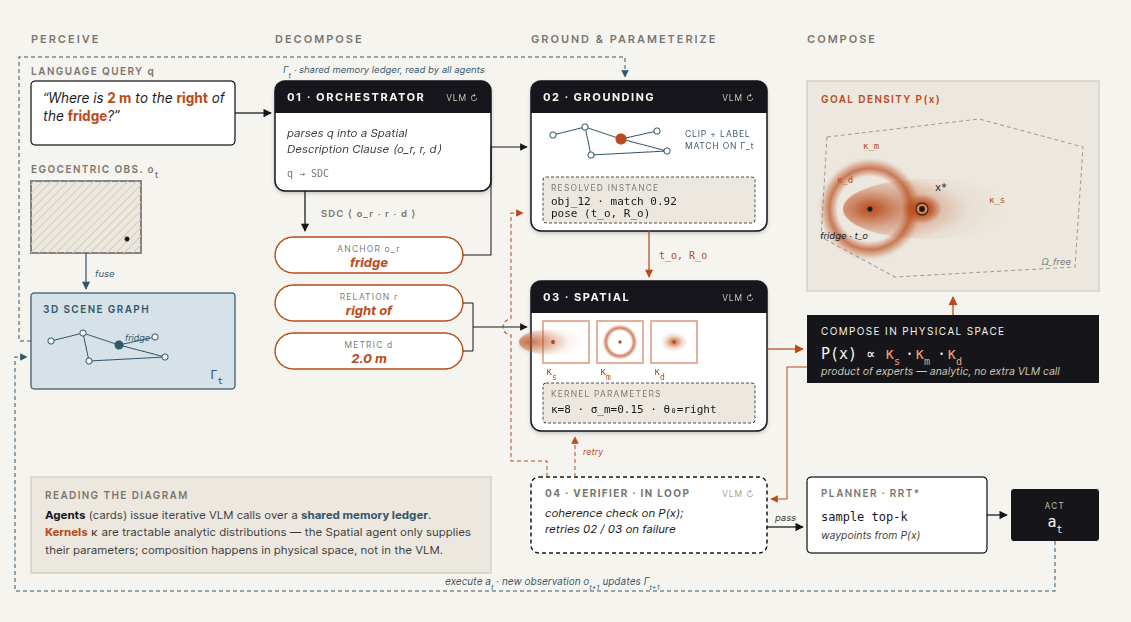
\includegraphics[width=0.99\linewidth]{figures/fig_3_system_overview.png}
    \caption{
      \textbf{MAPG system overview.}
      Egocentric observations $o_t$ are fused into a $3$D scene graph $\Gamma_t$, shared by all agents over a memory ledger.
      The Orchestrator parses the query $q$ into a Spatial Description Clause $\langle o_r, r, d\rangle$; the Grounding Agent resolves the referent $o_r$ against $\Gamma_t$; the Spatial Agent supplies parameters for the directional ($\kappa_s$), metric ($\kappa_m$), and anchor-density ($\kappa_d$) kernels.
      The kernels are composed analytically in physical space (a product of experts, no extra VLM call), yielding a goal density $P(x)$ over free space.
      The Verifier checks coherence and triggers corrective retries; on pass, the Planner samples top-$k$ waypoints to act, and the new observation updates $\Gamma_{t+1}$, closing the loop. \opnote{empty space}
      % \opnote{While I appreciate the effort, I'm not a fan of this figure. Can you please look at Figure 3 in GraphEQA paper and think if you can redesign this one similarly? Remember that your job through the image is not to convey the complexity of your method in its full glory, but to differentiate your method schematically from existing ways. Also you don't even talk about the verifier in your methods section. Perhaps also use this diagram to differentiate what you call an agent and what is a kernel.}
    }
    \label{fig:method_overview-h}
\end{figure*}



\section{Methodology}
%\ngnote{keep the methodology at about 1.5 pages. Right now you are at 2.5 pages. This is because you need space for the dataset as well. 2.5 pages will be gone to intro and related work.}
%\opnote{perhaps start with a problem formulation- what is the input output etc. single paragraph is good.}
% \opnote{I feel like this section misses several important points such as :1. perhaps motivate in a single line with why agentic? if it was agentic, what is a natural interface to combine the solution proposed by different agents? For example- language has been used to combine the output from multiple agents as done in \cite{du2024improving}, another popular way is using gradients as done in \cite{patil2025factorizingdiffusionpoliciesobservation}. Metric semantic language grounding presents us a unique problem where we can directly compose distributions in physical space- and hence we use analytical/tractable forms to leverage VLM's capabilities to infer the parameters. Then start talking about what agents you instantiate for functionally distinct roles and how you compose them in physical space. You also want to talk about parallels in input decomposition for better sample efficiency as done in \cite{du2024reducereuserecyclecompositional}.}

\noindent\textbf{Why an agentic decomposition?}
Multi-agent systems offer a natural interface when subproblems require specialist reasoning whose outputs must be combined into a shared representation. Prior work combines agent outputs via language~\cite{du2024improving} or gradients~\cite{patil2025factorizingdiffusionpoliciesobservation}. Metric-semantic goal grounding presents a unique opportunity: each subproblem (referent resolution, directional reasoning, metric estimation) produces a distribution over \emph{physical space}, so outputs compose directly as a Product of Experts~\cite{hinton2002poe, du2024compositionalgenerativemodelingsingle}, with no learned combiner required. Pre-specifying analytic kernel families mirrors the input-decomposition principle of~\cite{du2024reducereuserecyclecompositional}: each specialist VLM answers only the sub-question it handles best, concentrating capacity where it matters. We use \emph{agent} to mean a module that (a) receives a distinct subproblem, (b) iterates over evidence before returning, and (c) interfaces via structured output. The Orchestrator, Grounding Agent, and Verifier are genuine agents by this definition; the Spatial Kernel Estimator is a single-call parameterized kernel estimator.

\noindent\textbf{Problem Definition.}
Given a metric-semantic instruction $q$ and a partial $3$D scene graph $\Gamma=(V,E)$ with object nodes $V$, MAPG operates in two modes: \emph{object-to-world} (O-W), which infers a probability density $P(x \mid q, \Gamma)$ over allocentric waypoints $x \in \Omega_{\text{free}} \subset \mathbb{R}^3$; and \emph{object-to-object} (O-O), which selects among candidate object instances in $V$. In both modes, high-density regions correspond to locations satisfying the semantic referent, spatial predicate, and metric constraint specified in $q$. MAPG agents communicate through a shared blackboard storing the scene graph $\Gamma$, a referent belief $B_t$, an event ledger, and global failure history used for closed-loop refinement.
%\tn{is fig 2 referred to in the text anywhere?}
MAPG comprises the following components (Fig.~\ref{fig:method_overview-h}), drawing on the G$^3$ probabilistic grounding framework~\cite{tellex2011symbolgrounding}:\\

\begin{figure}[t]
    \centering
    \vspace{2mm}
    \begin{subfigure}[t]{0.45\linewidth}
        \centering
        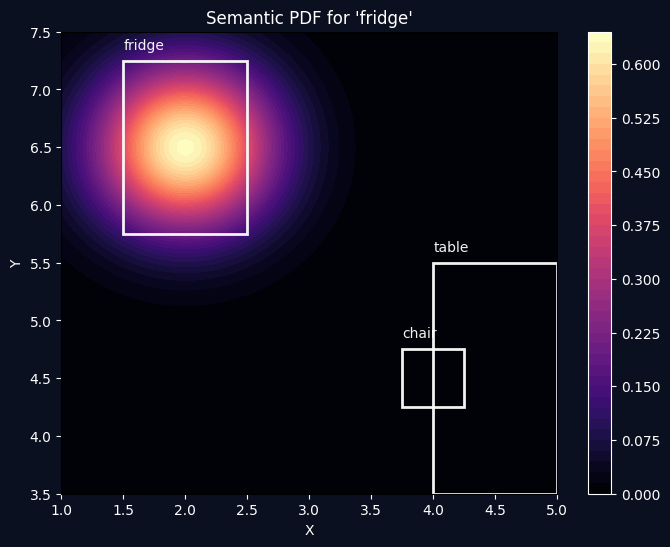
\includegraphics[width=0.95\linewidth]{figures/fridge_semantic.png}
        \caption{Semantic Grounding}
        \label{fig:fridge_semantic}
    \end{subfigure}\hfill
    \begin{subfigure}[t]{0.45\linewidth}
        \centering
        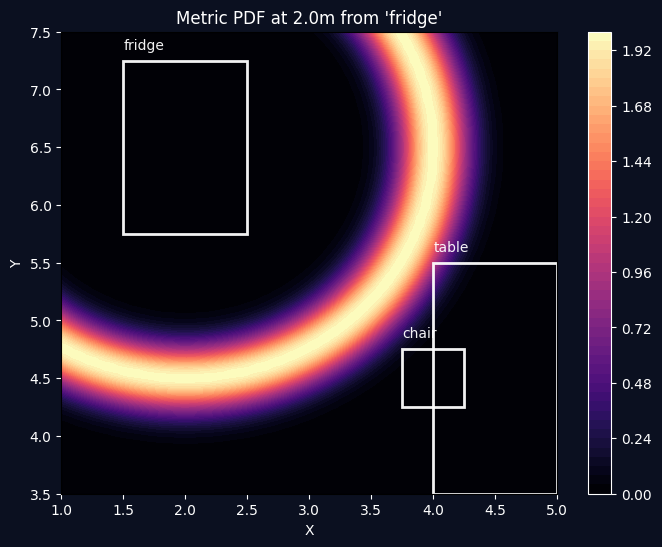
\includegraphics[width=0.95\linewidth]{figures/fridge_metric.png}
        \caption{Metric Kernel}
        \label{fig:fridge_metric}
    \end{subfigure}

    \vspace{0.3em}

    \begin{subfigure}[t]{0.45\linewidth}
        \centering
        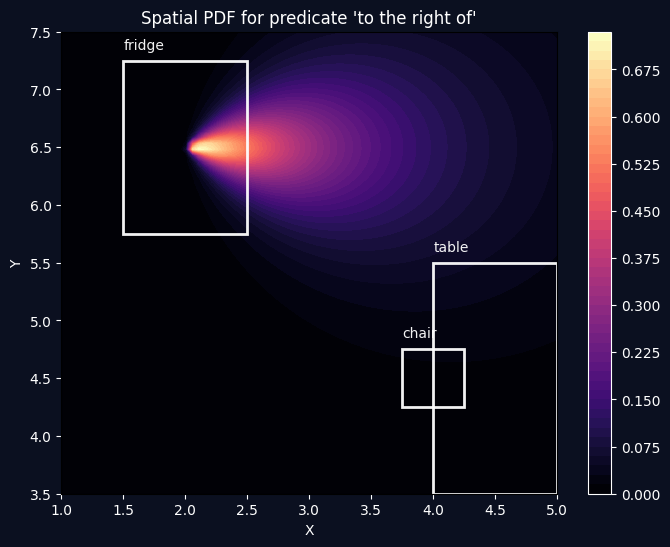
\includegraphics[width=0.95\linewidth]{figures/fridge_spatial.png}
        \caption{Spatial Kernel}
        \label{fig:fridge_spatial}
    \end{subfigure}\hfill
    \begin{subfigure}[t]{0.45\linewidth}
        \centering
        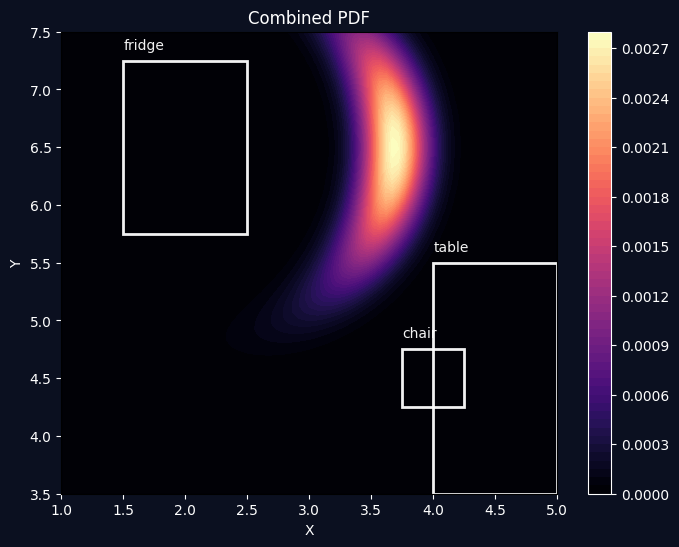
\includegraphics[width=0.95\linewidth]{figures/fridge_composed.png}
        \caption{Composed Distribution}
        \label{fig:fridge_composed}
    \end{subfigure}

    \caption{MAPG grounding for the query ``Where is \SI{2}{m} to the right of the fridge?'' Semantic grounding (a) identifies the fridge instance; the metric kernel (b) enforces the \SI{2}{m} radial offset; the directional kernel (c) captures ``right of'' as a vMF distribution in the fridge's local frame. Their log-space composition (d) yields a planner-ready goal distribution peaking $0.07\,\mathrm{m}$ from the ground truth.}
    \label{fig:fridge_kernels_row}
\end{figure}

%\opnote{My main complaint here is that the term agent has a specific meaning...}

\noindent$\!\!$\textbf{1) \uline{The Orchestrator}} parses a free-form instruction into Spatial Description Clauses (SDCs)~\cite{kollar2010toward}: a target entity, anchor objects with optional modifiers and explicit metric distances, and a \emph{composition logic} label. Crucially, the Orchestrator classifies each spatial predicate as either camera-relative (\texttt{near}, \texttt{between}) or intrinsic object-centric (\texttt{intrinsic\_front}, \texttt{intrinsic\_back}, \texttt{intrinsic\_left}, \texttt{intrinsic\_right}), enabling downstream kernel computation to select the correct reference frame. For ``Where is $2\,\mathrm{m}$ to the right of the fridge?'' it produces: anchor=\texttt{fridge}, composition\_logic=\texttt{intrinsic\_right}, metric=\texttt{2.0\,m}. Multi-clause instructions yield a conjunction of SDCs, each resolved independently and composed downstream.
%\opnote{The methods section is too mechanistic...}

\noindent$\!\!$\textbf{2) \uline{The Grounding Agent}} resolves each anchor label to a concrete object instance in $\Gamma$. Given a referent like ``fridge,'' it combines: (i) semantic equivalence matching (``couch'' = ``sofa'') against scene-graph labels, (ii) visual verification via a VLM query over base64-encoded egocentric images, and (iii) a spatial salience prior (proximity, visibility). Candidates rejected by the Verifier are blacklisted in the shared failure history and excluded from subsequent queries. A belief distribution $B_t(o)$ over candidate instances is maintained on the blackboard; the agent iterates across multiple views until sufficient confidence is reached, making it a genuine evidence-accumulating agent.

\rev{\noindent$\!\!$\textbf{3) \uline{Spatial Kernel Estimator}} (Spatial Agent)}: Once anchor $o_r$ with pose $t_o \in \mathbb{R}^3$ is resolved, MAPG instantiates three analytic kernels whose log-likelihoods sum in closed form (Fig.~\ref{fig:fridge_kernels_row}):

\noindent\textbf{Semantic kernel}: a $3$D Gaussian centered at the anchor: $\ell_{\text{sem}}(x) = -\tfrac{1}{2\sigma_s^2}\|x - t_o\|^2$.

\noindent\textbf{Metric kernel}: a radial Gaussian over distance from the anchor: $\ell_{\text{met}}(x) = -\tfrac{1}{2\sigma_m^2}(\|x-t_o\| - d_0)^2$, \rev{where $d_0$ is parsed from the query by the Orchestrator and $\sigma_m$ is a system tolerance.}

\noindent\textbf{Spatial (directional) kernel}: a von Mises-Fisher distribution~\cite{tellex2011symbolgrounding} in the anchor's local frame:
$\ell_{\text{dir}}(x;\theta_0,\phi_0,\kappa)=\kappa\bigl(R_o\,m(\theta_0,\phi_0)\bigr)^\top\widehat{(x-t_o)}$,
\rev{where $R_o$ maps from the anchor's local to world frame, $\widehat{(x-t_o)}$ is the unit direction from anchor to $x$, and $\kappa$ is a system concentration parameter.}

\rev{\noindent\textbf{Composition and the role of the semantic kernel.}
The three log-likelihoods sum and are normalized over $\Omega_{\text{free}}$. The semantic and metric kernels, however, are not independent: $\ell_{\text{sem}}$ is centred \emph{on} the anchor while $\ell_{\text{met}}$ peaks at radius $d_0$ \emph{from} it, so summing all three shrinks the composed mode inward. Along the modal ray $\ell_{\text{dir}}$ is constant in $r$, giving a closed form for the peak radius
\begin{equation}
r^{\star} = d_0\,\frac{\sigma_s^{2}}{\sigma_s^{2}+\sigma_m^{2}} \;<\; d_0 ,
\label{eq:shrinkage}
\end{equation}
a systematic underestimate of the commanded offset. With $\sigma_s$ scaled to the anchor extent ($\sigma_s=0.5\,\text{max-dim}$) and $\sigma_m=0.30\,\mathrm{m}$, a $2\,\mathrm{m}$ offset from a typical $0.8\,\mathrm{m}$ fridge would peak at $1.28\,\mathrm{m}$, an error of $0.72\,\mathrm{m}$ induced purely by the composition.
We therefore treat the semantic kernel as an \emph{anchor-selection} term rather than a goal-placement term. In O-O mode it scores candidate instances and all three kernels apply. In O-W mode, where the goal is a free-space waypoint and the anchor is already resolved, the semantic term carries no information about \emph{where along} the offset the goal lies, so we flatten it ($\sigma_s\!\to\!\infty$) and compose
\begin{equation}
\log P(x) = \ell_{\text{met}} + \ell_{\text{dir}},
\label{eq:ow-composition}
\end{equation}
which by Eq.~\ref{eq:shrinkage} recovers $r^{\star}=d_0$ exactly. This is what makes the metric constraint hold to centimetre accuracy; naively multiplying all three experts would not.}

\rev{\noindent\textbf{VLM parameter inference.} The Spatial Kernel Estimator prompts a VLM with the anchor label, current agent pose and yaw $\psi$, scene graph context, and an egocentric image. The VLM predicts the camera-relative azimuth $\theta_{\text{cam}}$ toward the goal region; the system converts this to a world-frame direction $\theta_0 = (\psi + \theta_{\text{cam}}) \bmod 2\pi$. For predicates classified as \texttt{intrinsic\_*} by the Orchestrator, $\theta_0$ is further resolved using the anchor's stored orientation rather than camera frame, enabling the commonsense subset's frame-of-reference predicates. This design asks the VLM only to answer ``in which camera direction is the goal?'' (a task VLMs handle well) while the coordinate transform and metric enforcement are handled analytically.}

\rev{\noindent$\!\!$\textbf{4) \uline{Cascading Spatial Kernels.}}
For compound instructions, one kernel triplet is instantiated per clause, each anchored to its resolved referent. All log-likelihoods are summed and renormalized, implementing a Product of Experts~\cite{hinton2002poe} whose peak satisfies the conjunction of all spatial constraints.}

\rev{\noindent$\!\!$\textbf{5) \uline{Verifier and Planner.}}
The \emph{Verifier} performs four checks on each proposed grounding: (i) orchestrator logic soundness, (ii) egocentric alignment ($\theta_{\text{cam}}$ consistent with what is visible in the image), (iii) semantic label flexibility (``sofa'' accepted for ``couch''), and (iv) absence of visual hallucination. A FAIL result appends structured feedback to the global failure history and re-triggers the Grounding Agent or Spatial Kernel Estimator as appropriate, forming a closed refinement loop. Waypoints that pass verification are forwarded to the \emph{Planner} (RRT*~\cite{karaman2011sampling}) for trajectory generation.}

\section{Datasets}
\label{sec:datasets}

Several benchmarks study spatial reasoning, including SpatialRGPT-Bench~\cite{spatialRGPT} and $3$DSRBench~\cite{3dsrbench}, but their primary modality is single-image VQA, which precludes evaluation of (i) viewpoint consistency, (ii) partial observability, and (iii) the need for exploration before committing to an answer. Embodied QA benchmarks such as HM-EQA~\cite{ren2024exploreconfidentefficientexploration}, used as an evaluation set by systems like GraphEQA~\cite{graphEQA}, %\opnote{HM-EQA is not from graph-EQA?? also GraphEQA is not a benchmark?}
move closer by emphasizing interaction and persistent memory, but target semantic or factual questions rather than \emph{metric--semantic--predicate} grounding (e.g., ``$2\,\mathrm{m}$ left of the chair'') as an evaluation target.

To isolate $3$D metric goal grounding, we introduce \textbf{MAPG-Bench} (Map-based Anchored Predicate Grounding Benchmark). MAPG-Bench contains $98$ human-annotated queries across $41$ HM$3$D~\cite{ramakrishnan2021habitatmatterport3ddatasethm3d} indoor scenes rendered in Habitat-Sim. %\opnote{How many queries in total??? Are all metric or are some object based too?}
It comprises two complementary query types: \textbf{Object-to-World (O-W)} queries require localizing a continuous $3$D allocentric waypoint relative to an anchor object (e.g., ``Where is $2\,\mathrm{m}$ to the right of the fridge?''), and \textbf{Object-to-Object (O-O)} queries require selecting the correct instance among multiple candidates satisfying a relational predicate (e.g., ``Which chair is in front of the sofa?''). 
% \opnote{If you have both- you need to introduce O-O and O-W here and specify how many of both are present in the dataset. If not you're good. This is important cause you liberally use O-O and O-W without introducing them formally as a part of your benchmark. You also need to say where those terms come from (cite the paper).}

Annotations were collected with an interactive tool that overlays semantic instance labels on the agent's egocentric view. Annotators explored each scene, selected anchor instances, and recorded the agent's pose. For O-W queries, the ground truth is an explicit $3$D allocentric point placed on a navigable surface, an actionable waypoint rather than a text description. Predicates cover three families: horizontal directional (\texttt{in-front-of} $33$, \texttt{right-of} $18$, \texttt{behind} $13$, \texttt{left-of} $11$), vertical (\texttt{above} $10$, \texttt{below} $4$), and relational (\texttt{between} $6$, \texttt{near} $1$, \texttt{towards} $1$, \texttt{from} $1$). Metric distances span typical indoor scales ($0.5$--$4.0\,\mathrm{m}$); a further $6$ queries carry no metric offset ($d_0=0$) and serve as purely directional controls. A specialized \emph{commonsense} subset probes VLM failures on intrinsic frame-of-reference predicates, where the ``front'' of an object is defined by its affordance direction rather than the camera's line of sight, a systematically hard case documented in~\cite{frameOfReferenceAmbiguity}.

\begin{figure}[!t]
  \centering
  \vspace{2mm}
  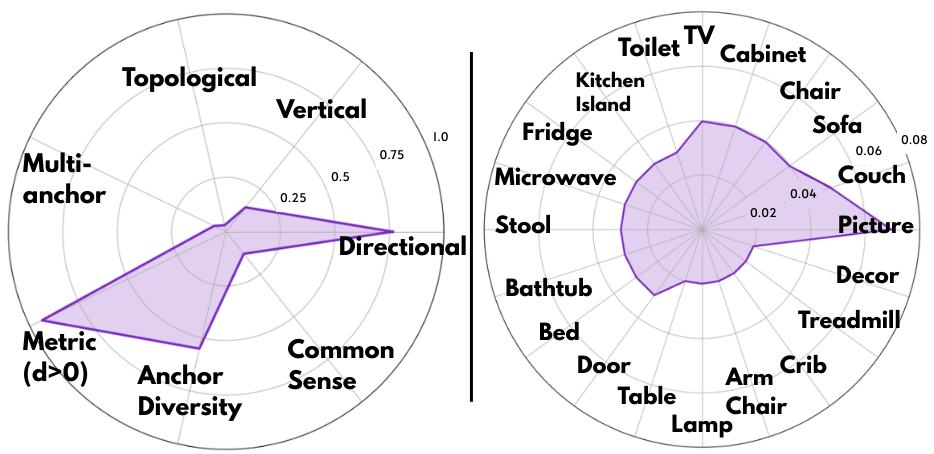
\includegraphics[width=0.90\linewidth,height=10cm,keepaspectratio]{figures/fig_5.png}
  \caption{\textbf{Distribution} of query categories (left) and anchor object labels (right) in MAPG-Bench. \rev{Example queries: (O-W, metric) ``Where is $2\,\mathrm{m}$ to the right of the fridge?''; (O-W, directional) ``Where is directly behind the sofa?''; (O-O) ``Which chair is nearest to the window?''; (commonsense) ``Where is in front of the armchair?'' (resolved via affordance direction).} %\opnote{IMP: You should extend this figure and how 3-4 examples of the queries you have added in mapg-bench. This can go in the caption too.}
  }
  \label{fig:mapg_distributions}
\end{figure}
\section{Experimental Results}
\label{sec:experiments}


\begin{table*}[t]
\vspace{4pt}
\centering
\small
\setlength{\tabcolsep}{5pt}
\renewcommand{\arraystretch}{1.15}

\resizebox{\linewidth}{!}{
\begin{tabular}{lcccccccc}
\toprule
\textbf{Method}
& \textbf{$d$ Err. O-O $\downarrow$} & \textbf{$d$ Err. O-W $\downarrow$}
& \textbf{Angle Err. $\downarrow$}
& \textbf{Obj. Sel. $\uparrow$} & \textbf{Common Sense $\uparrow$}
& \textbf{TSR $\uparrow$} & \textbf{Anchor Pick SR $\uparrow$} & \textbf{Avg. Traj. Len $\downarrow$} \\
& \textbf{(\si{\meter})} & \textbf{(\si{\meter})}
& \textbf{(\si{\degree})}
& \textbf{(Acc.)} & \textbf{(Acc.)}
& \textbf{(Rate)} & \textbf{(Rate)} & \textbf{(\si{\meter})} \\
\midrule

\multicolumn{9}{l}{\textbf{Open-Sourced Specialist}} \\
\midrule
SRGPT (SpatialRGPT-7B)  & $0.50$ & N/A    & $10.00$ & $0.36$ & N/A    & N/A    & N/A    & N/A   \\
GraphEQA (Gemini 2.5 Pro) & N/A  & $5.82$ & $30.78$ & $0.34$ & $0.14$ & $0.78$ & $0.48$ & $1.32$ \\
\midrule

\multicolumn{9}{l}{\textbf{Ours}} \\
\midrule
MAPG (Gemini 3 Pro)       & $0.58$ & $\textbf{0.08}$ & $15.13$ & $0.30$ & $0.14$ & $0.46$ & $0.46$ & $14.60$ \\

MAPG (OpenAI GPT 5.2)     & $0.42$ & $\textbf{0.07}$ & $\textbf{4.79}$ & $0.28$ & $0.16$ & $\textbf{0.98}$ & $\textbf{0.98}$ & $\textbf{1.30}$ \\

MAPG (Gemini 2.5 Pro)     & $0.08$ & $0.45$ & $6.19$ & $\textbf{0.42}$ & $0.08$ & $0.90$ & $0.94$ & $2.50$ \\

MAPG (Claude Opus 4.6) & $\textbf{0.07}$ & $0.43$ & $10.30$ & $0.36$ & $\textbf{0.30}$ & $0.806$ & $0.816$ & $4.33$ \\
\bottomrule
\end{tabular}
}

\caption{Comparison of MAPG against scene-graph EQA and single-image spatial-reasoning baselines on \textbf{MAPG-Bench}.
Proprietary generalist models were benchmarked; they exhibit inconsistent performance and do not reliably produce actionable $3$D goals across tasks, so we omitted them for space (available on our website).
Metrics with $\uparrow$ are higher-is-better; $\downarrow$ are lower-is-better.
\textbf{Obj.\ Sel.} measures whether the predicted target object satisfies the spatial query in O-O grounding, evaluated independently of navigation success.
\textbf{Angle Err.} is the combined directional error between the predicted and ground-truth offset directions, computed as angle $\Delta = \arccos\!\big(\cos(\text{yaw err})\cos(\text{pitch err})\big)$ over the unit sphere.
\textbf{TSR} measures end-to-end instruction completion, including both grounding and navigation.
\textbf{Common Sense} measures accuracy on a specialized subset probing intrinsic frame-of-reference predicates (e.g., ``in front of'' resolved using object affordance direction rather than camera direction).
\textbf{Anchor Pick SR} measures anchor instance disambiguation under partial observability.
\textbf{Avg.\ Traj.\ Len} measures behavioral efficiency.
$^{\dagger}$We did not run GraphEQA with Claude Opus 4.6 due to API cost constraints; this comparison is a direction for future work.
}

% \opnote{several complaints here: 1. do not have different precision in numbers. if  something is 1.80, then write it as 1.80 and not 1.8 . All results should have two decimal places. 2. Why is MAPG Gemini pro so bad in avg traj len?? Seems like it is low on achor pick SR too- why is it worse than Gemini 2.5 pro??? Gemini 3 should be better than 2.5 right? 3. What is common sense Acc?? 4. Specify the VLM used for SRGPT and GraphEQA. 5 Why is object selection accuracy low but TSR high?}
%tn{Common Sense is now defined in the caption above}
\label{tab:mapg_bench}
\end{table*}

% \opnote{this section need not be separate, and you can talk about your experimental setup along with the results, but it is also okay to keep if you have space.}
%\opnote{This section can be organized better- for example: each paragraph can say a separate thing- one for metrics, one for what you're trying to evaluate, one for baselines etc. Bold the first word of each para that is representative of what the para is trying to say. for example: \textbf{Baselines.} We report results on ...}
\textbf{Task.} We evaluate \emph{goal grounding} under a common requirement: given a spatial query, egocentric observations, and a persistent $3$D scene representation (scene graph), the system must output a grounded target that is directly usable by a planner. Depending on the query type, the output is either (i) an \emph{allocentric waypoint} for object-to-world (O-W, \emph{``Where''}) queries or (ii) an \emph{object selection} for object-to-object (O-O) queries. %\opnote{write the shorthand you use O-W or O-O in your tables}
Our evaluation isolates whether a method can (a) resolve the intended anchor under ambiguity, (b) interpret predicates in a consistent frame of reference, and (c) satisfy explicit metric constraints, while remaining robust under viewpoint changes and partial observability. 



\textbf{Metrics.} On MAPG-Bench we report both geometric error and task-level success. We measure distance error for O-O and O-W grounding (meters) and yaw/pitch angular error (degrees) to quantify directional consistency of the predicted offset. For O-O cases, we report object-selection accuracy using embedding-based soft matching between predicted and ground-truth object names to account for label-space mismatches between HM$3$D annotations and Hydra-derived semantic classes; MAPG is scored using the best match over its ranked Top-1/Top-2 predictions. For embodied efficiency, we report TSR, anchor-pick success rate (instance disambiguation under partial observability), and average trajectory length (meters).
%We report mean $\pm$ SEM (standard error of the mean, $\sigma / \sqrt{n}$) across queries. \opnote{I'm sus about the yaw pitch degrees- have you seen other papers do that?} %\opnote{I don't understand this- what is identification style cases? is this O-O or O-W?} %\opnote{Not sure what this means}

\textbf{Baselines.} We compare MAPG against scene-graph EQA (GraphEQA) and single-image spatial specialists (SpatialRGPT). We modified GraphEQA's planner interface to answer spatial ``where'' questions by producing a text waypoint from the scene graph, yielding a fair scene-graph-driven baseline for metric-semantic grounding. We evaluate multiple MAPG variants that share the same distributional grounding pipeline but differ only in the underlying VLM backend, isolating the effect of model choice from pipeline structure.

\textbf{Completed end-to-end run.}
The completed evaluation used the Claude Opus 4.6 planner model, seed $42$, the \texttt{bench\_v1\_98} split, and llvmpipe software rendering with \texttt{sim\_gpu=-1}. All $98$ episodes completed. MAPG succeeded on $79$ episodes ($80.6\%$), and the anchor was found on $80$ ($81.6\%$). Mean steps and mean trajectory length were both $4.33$. The run made $830$ model calls, including $142$ retries, all of which were flagged; every call had a usage row, and total spend was \$15.780490 against a \$25 cap.
During the run, an out-of-range Habitat semantic instance ID stopped question index $95$; commit \texttt{c1b1ee5e} sanitized only out-of-range IDs, and the same run was resumed in place rather than restarted after validating the seed, split, and configuration hashes.

\begin{table*}[t]
\centering
\small
\begin{minipage}[t]{0.48\textwidth}
\centering
\begin{tabular}{lrr}
\toprule
\textbf{Predicate} & \textbf{$n$} & \textbf{Success} \\
\midrule
above       & 10 & 9 ($90.0\%$) \\
behind      & 13 & 10 ($76.9\%$) \\
below       & 4  & 1 ($25.0\%$) \\
between     & 6  & 3 ($50.0\%$) \\
from        & 1  & 1 ($100\%$) \\
in front of & 33 & 27 ($81.8\%$) \\
left of     & 11 & 10 ($90.9\%$) \\
near        & 1  & 1 ($100\%$) \\
right of    & 18 & 16 ($88.9\%$) \\
towards     & 1  & 1 ($100\%$) \\
\bottomrule
\end{tabular}
\caption{Success in the completed run, grouped by predicate.}
\label{tab:predicate_success}
\end{minipage}
\hfill
\begin{minipage}[t]{0.48\textwidth}
\centering
\begin{tabular}{lrr}
\toprule
\textbf{Target distance} & \textbf{$n$} & \textbf{Success} \\
\midrule
$0\,\mathrm{m}$   & 6  & 3 ($50.0\%$) \\
$0.5\,\mathrm{m}$ & 19 & 14 ($73.7\%$) \\
$1\,\mathrm{m}$   & 34 & 28 ($82.4\%$) \\
$1.2\,\mathrm{m}$ & 1  & 1 ($100\%$) \\
$1.5\,\mathrm{m}$ & 12 & 10 ($83.3\%$) \\
$2\,\mathrm{m}$   & 20 & 18 ($90.0\%$) \\
$2.5\,\mathrm{m}$ & 3  & 3 ($100\%$) \\
$3\,\mathrm{m}$   & 1  & 1 ($100\%$) \\
$4\,\mathrm{m}$   & 2  & 1 ($50.0\%$) \\
\bottomrule
\end{tabular}
\caption{Success in the completed run, grouped by target distance.}
\label{tab:distance_success}
\end{minipage}

\vspace{3pt}
\parbox{\textwidth}{\footnotesize\textbf{Interpretation.}
Tables~\ref{tab:predicate_success} and~\ref{tab:distance_success} are descriptive breakdowns of one split. \texttt{below} has $1$ success in $4$ examples ($25.0\%$), and \texttt{between} has $3$ in $6$ ($50.0\%$). These cells are hypotheses for follow-up, not stable conclusions. Several predicate and distance cells contain only one to three examples, so their percentages should not be generalized.}
\end{table*}

\textbf{Rendering fallback disclosure.}
The original run log contains $35$ black-render fallback markers affecting split indices $14$, $38$, and $39$. When every sampled image in an affected camera batch was filtered as black, the system used the final unfiltered raw image. Two of the three affected episodes succeeded. Excluding all three gives $77$ successes in $95$ episodes ($81.1\%$), compared with $79$ in $98$ ($80.6\%$) for the full result. This sensitivity check does not show that the fallback caused or prevented any outcome.

\noindent A) \textbf{MAPG-Bench results:}
% \opnote{Don’t start with the entre- remind the reader what the benchmark evaluates and what grounding skills are needed to do well in it. Start by talking about O-O results cause similar problems already exist in other benchmarks (ignore if irrelevant)? Talk about results on sub components fromt he table- why is anchor selection accuracy low of graphEQA? Then come to the main result.}
MAPG-Bench evaluates three grounding skills jointly: anchor instance disambiguation (Anchor Pick SR), predicate interpretation in a consistent allocentric frame (yaw/pitch error), and metric constraint satisfaction (O-W error). Table~\ref{tab:mapg_bench} reports quantitative performance. To illustrate the contrast, consider the query ``Where is $2\,\mathrm{m}$ to the right of the fridge?’’ GraphEQA selects the scene-graph node with the nearest bounding box satisfying the directional predicate, without enforcing the metric offset; the resulting waypoint is $5.82\,\mathrm{m}$ from the ground truth. MAPG’s Orchestrator extracts \{anchor: \texttt{fridge}, predicate: \texttt{right-of}, metric: $2.0\,\mathrm{m}$\}; the Grounding Agent resolves the fridge instance from the scene graph; the Spatial Kernel Estimator instantiates a vMF directional kernel ($\theta_0 = 90^\circ$ in the fridge’s local frame) and a radial Gaussian metric kernel ($d_0 = 2.0\,\mathrm{m}$, $\sigma_m = 0.30\,\mathrm{m}$); the composed distribution peaks $2.04\,\mathrm{m}$ to the right of the fridge, yielding a waypoint $0.07\,\mathrm{m}$ from the ground truth (see Fig.~\ref{fig:fridge_kernels_row}).

GraphEQA exhibits a large O-W distance error ($5.82\,\mathrm{m}$) and high angular inconsistency ($13.50^\circ$ yaw, $27.90^\circ$ pitch), reflecting its tendency to select the nearest region satisfying a predicate without enforcing the metric offset. Its Anchor Pick SR ($0.48$) is also substantially lower than MAPG’s best ($0.98$), showing that committing early to a single scene-graph query under partial observability misses the correct instance roughly half the time \opnote{what does this mean?}. MAPG (OpenAI GPT-5.2) reduces O-W error from $5.82\,\mathrm{m}$ to $0.07\,\mathrm{m}$ (98.8\% reduction, SEM $0.03\,\mathrm{m}$), yaw error from $13.50^\circ$ to $1.90^\circ$ (85.9\% reduction), and pitch error from $27.90^\circ$ to $4.40^\circ$ (84.2\% reduction), while achieving $0.98$ TSR and $0.98$ anchor-pick SR with short trajectories ($1.30\,\mathrm{m}$). These gains follow directly from MAPG’s two design novelties: (i) explicit query decomposition (anchor / predicate / metric) and (ii) probabilistic composition of per-clause kernels into a planner-queryable goal distribution. \opnote{you need to say how/why it follows from those decisions.}
%\opnote{IMP: Add an example of a query where MAPG does better than the baseline and talk about where the baseline examtly fails- the failure mode of the baseline and why MAPG succeeds.}

On O-O grounding, SpatialRGPT achieves $0.50\,\mathrm{m}$ error, consistent with its ability to reason about directional relations from a single image. However, when the target object is not visible in the best single view or requires integrating evidence across multiple viewpoints, SRGPT has no mechanism to resolve the discrepancy. MAPG (Claude Opus 4.6) reaches $0.07\,\mathrm{m}$ O-O error (86\% reduction vs SRGPT), because the Grounding Agent accumulates multi-view evidence before committing to the anchor instance, and the Spatial Kernel Estimator composes a $3$D belief anchored to the resolved object pose rather than a single-frame estimate \opnote{I don't understand this}. 
% \opnote{perhaps start with this paragraph. IMP: Also you need to be more detailed here- give an example where SRGPT fails and you succeed. You need to better explain why your method succeeds- your explanation does not talk about why your method is better, and that is important.}

This trade-off reflects the different demands of each task type: O-O grounding is primarily a disambiguation problem requiring accurate semantic matching and visual evidence accumulation across views, where Claude Opus 4.6’s strong CLIP-based referent resolution yields the lowest O-O error ($0.07\,\mathrm{m}$). O-W grounding additionally requires predicting precise metric offset parameters $(d_0, \sigma_m)$ from a spatial predicate, where GPT-5.2’s superior instruction-following on structured spatial prompts produces better-calibrated metric kernels and the lowest O-W error ($0.07\,\mathrm{m}$). \opnote{I also don't understand this.}
% \opnote{Why? You cannot get away with simply saying this- you need to justify why this is happening}
MAPG (Gemini 3 Pro) exhibits higher trajectory length and lower anchor-pick SR than MAPG (Gemini 2.5 Pro), consistent with Gemini 3 Pro being a preview checkpoint with weaker instruction-following on structured spatial prompts; we retain it for completeness \opnote{this is not a valid argument}. The overall pattern persists across all MAPG variants: low metric error and improved directional consistency versus the scene-graph baseline, validating that the \emph{pipeline structure} (decomposition + composition) is the primary driver of spatial grounding performance. 
% \opnote{the reason for performance improvement is not clear through your explanations, and adding actual examples and failure modes of the baselines will help a lot.}

\noindent B) \textbf{HM-EQA Results (Generality without metric constraints):} 
% \opnote{This needs to be separate subsection, and you need to write this as- our method also results in improved or equivalent performance on existing EQA benchmarks that do not necessarily involve metric constraints, highlighting its generality and broad applicability.}
To assess whether MAPG's metric-semantic decomposition degrades performance on tasks without metric constraints, we evaluate on HM-EQA~\cite{ren2024exploreconfidentefficientexploration}, a semantic QA benchmark over HM3D scenes introduced by Explore-EQA where success is measured by multiple-choice answer accuracy over object properties and states complementary to MAPG-Bench's continuous goal-grounding evaluation. 
% \opnote{This cannot be the description of the benchmark. What is it designed to measure and how it is different from our MAPG benchmark? How it calculate success doe not merit a mention here.} 

\begin{table}[t]
\centering
\footnotesize
\setlength{\tabcolsep}{5pt}
\renewcommand{\arraystretch}{1.03}

\begin{tabular}{p{4.8cm}cc}
\toprule
\multicolumn{3}{c}{\textbf{Benchmarking on HM-EQA Question Answering}} \\
\midrule
\textbf{Method} & \textbf{TSR $\uparrow$} & \textbf{$L_{\tau}$ (\si{\m}) $\downarrow$} \\
\midrule

Explore-EQA & $0.52$ & $38.1$ \\
Explore-EQA-GPT4o & $0.46$ & $6.3$ \\
Explore-EQA-Llama4-Mav & $0.44$ & $10.4$ \\
Explore-EQA-Gemini-2.5Pro & $0.54$ & $12.3$ \\
GraphEQA-Gemini-2.5Pro & $\textbf{0.67}$ & $7.41$ \\
GraphEQA (Gemini 2.5 Pro)$^{+}$ & $0.61$ & $5.48$ \\
GraphEQA (GPT 5.2)$^{+}$ & $0.63$ & N/A \\
MAPG (OpenAI GPT 5.2) (Ours) & $0.60$ & N/A \\
MAPG (Claude 4.6 Opus) (Ours) & $\textbf{0.71}$ & $6.62$ \\
\bottomrule
\end{tabular}
\caption{EQA question-answering accuracy on HM-EQA~\cite{ren2024exploreconfidentefficientexploration}. $^{+}$ indicates our implementation of the particular baseline. MAPG achieves higher TSR while carrying out more exploration before committing to the target, consistent with its evidence-accumulation design. A GraphEQA + Claude Opus 4.6 comparison was omitted due to API cost constraints and is a direction for future work. %\opnote{Why have you not baselined graph eqa with claude also? How do you know your performance is not simply due to a stronger MLLM/VLM backend?}
\opnote{this reasoning is not acceptable.}
}
\label{tab:eqa_qa_accuracy}
\end{table}

Table~\ref{tab:eqa_qa_accuracy} reports QA accuracy. Our method achieves improved or equivalent performance on HM-EQA, highlighting its generality and broad applicability even when metric constraints are absent. MAPG (Claude Opus 4.6) reaches $0.71$ TSR, outperforming GraphEQA-Gemini-2.5Pro ($0.67$) and all Explore-EQA variants ($0.44$--$0.54$). This indicates that MAPG's evidence-accumulation loop and anchor disambiguation, when decoupled from metric kernel prediction, transfer effectively to semantic QA tasks. We use HM-EQA as a complementary diagnostic, while MAPG-Bench remains our primary evaluation for metric-semantic goal grounding.

\noindent C) \textbf{Ablations:}
% \label{subsec:ablations_results}
We ablate MAPG to quantify why explicit spatial reasoning and modular agents are necessary. Table~\ref{tab:ablations_spatial} shows that removing the explicit spatial reasoner (replacing it with a single ``fat'' planner with curated chain-of-thought) drops object selection SR from $0.42$ to $0.20$ over the full $n=98$ benchmark (Fisher exact $p<10^{-3}$), while the full MAPG configuration improves over the GraphEQA base ($0.34$ to $0.42$). These results support the claim that \emph{explicit composition of metric and predicate constraints} is not recoverable from prompting alone, consistent with the running fridge example, where CoT-only reasoning misses the $2\,\mathrm{m}$ offset entirely. %\opnote{add an example failure- like refer to objects- or have a running example through the paper.}

We further evaluate robustness under uncertainty induced by occlusion. In Table~\ref{tab:ablations_occlusion}, the explicit spatial reasoner improves object selection SR from $0.30$ to $0.50$ under occlusion, suggesting that maintaining intermediate belief over anchors and deferring commitment can recover from partial observability when the anchor eventually enters the map. We report this as a qualitative indication rather than a statistical result: the occlusion subset contains only $n=10$ queries over $5$ scenes, so the difference amounts to two queries (Fisher exact $p=0.65$) and is not significant. Enlarging this subset is ongoing work.

The commonsense-focused subset probes frame-of-reference predicates where the correct interpretation requires reasoning about intrinsic object orientation (e.g., the ``front’’ of a chair is the side facing a seated occupant, not the camera’s front). On this subset (Table~\ref{tab:mapg_bench}, Common Sense column), MAPG (Claude Opus 4.6) achieves $0.30$ accuracy, more than doubling the GraphEQA baseline ($0.14$). This gain reflects MAPG’s explicit predicate decomposition: rather than asking a single model to jointly resolve the referent and interpret the predicate, MAPG’s Grounding Agent first resolves the anchor instance and the Spatial Kernel Estimator separately reasons about the directional predicate in the anchor’s local frame. The remaining gap from perfect accuracy reflects the difficulty of intrinsic object-orientation inference from partial views, a target for future work in richer scene representations. 
\opnote{para not clear.} 
%\opnote{this whole paragraph is bad news. One you cannot talk about abstract things without making the reader understand what youa re talking about with at elast a few concrete examples. Two- I see in table 1 that we do equal or better than the baselines? 3 the conclusion you have derived here does not help your case at all.}

\noindent D) \textbf{Real-World Demonstration:} %\opnote{Not sure what you are talking about here- you need to provide more details for everything- what was the task, what was the query- what did the robot do etc. I'm not saying you eat away many lines of this section- but add details in a dense manner. One line with all the details should do, or at least write please see figure 6 for task and query details}
Using a Robotis AI Worker robot, we built an offline $3$D scene graph from RGB-D observations of a physical lab environment and evaluated MAPG on three spatial queries, including ``Where is $1\,\mathrm{m}$ to the right of the trash can near the bicycle?'' MAPG resolved the correct anchor instance amid distractors, composed a spatial distribution peaking at the annotated target region (see Fig.~\ref{fig:obs-anchor-trace}), and produced a planner-ready waypoint within the expected tolerance. These results indicate that MAPG transfers to physical environments when a structured scene representation is available, though systematic real-world benchmarking is deferred to future work. A video of the demonstration is provided in the supplementary material.

\begin{table}[t]
\centering

\renewcommand{\arraystretch}{1.1}
\setlength{\tabcolsep}{6pt}


\begin{tabular}{l c}
\toprule
% \multicolumn{2}{c}{\textbf{Ablation Spatial reasoner}} \\
% \midrule
\textbf{Method} & \textbf{Object selection SR $\uparrow$} \\
\midrule
GraphEQA (base)                          & $0.34$ \\
MAPG (CoT w/o spatial reasoner)            & $0.20$ \\
MAPG (explicit spatial reasoner)         & $0.42$ \\
\bottomrule
\end{tabular}


\caption{Replacing the explicit spatial reasoner with CoT degrades object selection success rate, while the full MAPG variant achieves the best performance. }
\label{tab:ablations_spatial}
\end{table}




\begin{table}[t]
\centering

\renewcommand{\arraystretch}{1.1}
\setlength{\tabcolsep}{6pt}


\begin{tabular}{l c}
\toprule
% \multicolumn{2}{c}{\textbf{Ablations: Occlusion (MAPG)}} \\
% \midrule
\textbf{Method} & \textbf{Object selection SR $\uparrow$} \\
\midrule
GraphEQA (base)                          & $0.30$ \\
MAPG (CoT- w/o spatial reasoner)            & $0.30$ \\
MAPG (explicit spatial reasoner)         & $0.50$ \\
\bottomrule
\end{tabular}


\caption{Occlusion highlights the limits of CoT-only reasoning, while the full MAPG variant performs best.}
\label{tab:ablations_occlusion}
\end{table}






% \begin{table}[t]
% \centering
% \renewcommand{\arraystretch}{\tblstretch}
% \setlength{\tabcolsep}{6pt}

% \begin{tabular}{l c}
% \toprule
% \multicolumn{2}{c}{\textbf{Ablation: Commonsense (MAPG)}} \\
% \midrule
% \textbf{Method} & \textbf{Commonsense object selection SR $\uparrow$} \\
% \midrule
% GraphEQA (base)                  & $0.30$ \\
% MAPG (OpenAI GPT-5.2) (Ours)     & $0.40$ \\
% MAPG (Gemini 2.5 Pro) (Ours)     & $0.30$ \\
% MAPG (Claude 4.6 Opus) (Ours)    & $0.60$ \\
% \bottomrule
% \end{tabular}


% \caption{Commonsense-focused object selection success rate (SR). Higher is better.}
% \label{tab:ablations_commonsense}
% \end{table}


\begin{figure*}[!t]
  \centering
  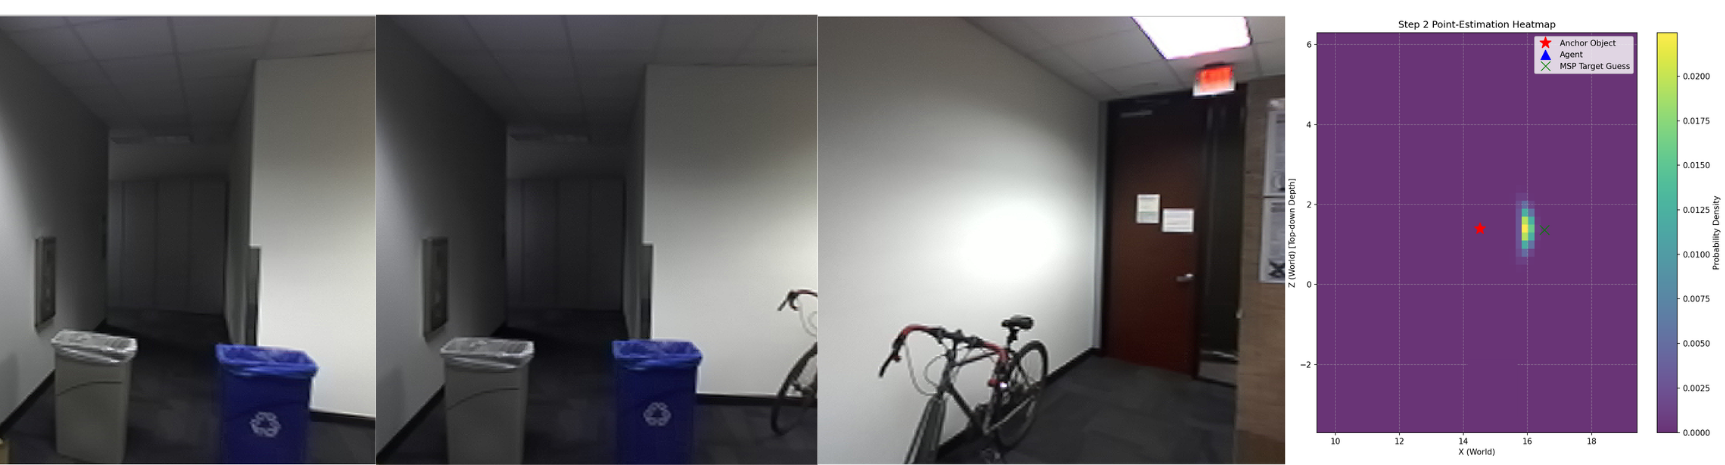
\includegraphics[width=\textwidth]{figures/fig_6_robot.png}
  \caption{\rev{\textbf{Real-world MAPG grounding example.} Using observations collected from a Robotis AI Worker robot, we construct an offline scene graph of a physical indoor environment. Three egocentric image frames are shown, with the query ``Where is $1$ meter to the right of the trash can close to the bicycle?'' MAPG infers a spatial probability distribution over candidate goal locations (right). The anchor (red) and predicted goal (green) illustrate metrically consistent semantic grounding in a physical environment: the grounded area is $1\,\mathrm{m}$ to the right of the blue trash can, consistent with the bicycle's position.}}
  \label{fig:obs-anchor-trace}
\end{figure*}

\section{Observations and Discussions}
\label{sec:observations}
% \opnote{IMP: need more numbers everywhere, even in the text. ...}
%\opnote{Lots of redundant stuff in this section. You should make it denser.}

The completed Claude Opus 4.6 run succeeded on $79$ of $98$ episodes ($80.6\%$) and found the anchor on $80$ ($81.6\%$). Tables~\ref{tab:predicate_success} and~\ref{tab:distance_success} provide the corresponding breakdowns, with the small-cell caution stated alongside them.
Tables~\ref{tab:mapg_bench}--\ref{tab:ablations_occlusion} show that MAPG's gains stem from two design choices:
% \opnote{bad language, say improvements are shown through results and point to tables.}
\textbf{(i) query decomposition} (anchor / predicate / metric) and \textbf{(ii) probabilistic composition} of per-clause kernels into a planner-queryable goal density. On MAPG-Bench, MAPG (GPT-5.2) reduces O-W error from $5.82\,\mathrm{m}$ to $0.07\,\mathrm{m}$ and improves TSR from $0.78$ to $0.98$. Ablations in Tables~\ref{tab:ablations_spatial} and~\ref{tab:ablations_occlusion} show %\opnote{bad language. Ablations in Table XYZ show that ...}
that these gains are primarily due to our compositional framework 
% \opnote{primarily due to our compositional framework}
rather than ``better prompting'': removing the spatial reasoner drops object-selection SR from $0.42$ to $0.20$, and under occlusion, explicit reasoning recovers SR from $0.30$ to $0.50$.

\noindent\textbf{Multi-view evidence accumulation enables reliable anchor disambiguation.}
The Grounding Agent iterates over egocentric views, accumulates CLIP-scored evidence, and maintains a blacklist of Verifier-rejected candidates, deferring commitment until confidence exceeds threshold. This behavior directly explains MAPG's high Anchor Pick SR (up to $0.98$, vs.\ GraphEQA's $0.48$). GraphEQA selects the nearest scene-graph match at the first step; under partial observability this commits to the wrong instance roughly half the time. The occlusion ablation confirms this: when the anchor is initially occluded, MAPG's iterative belief update recovers upon re-observation, whereas CoT-only reasoning has no mechanism to revise its initial commitment.

\noindent\textbf{Log-space kernel composition yields planner-ready allocentric waypoints.}
MAPG's final waypoint is the peak of a composed density over $\Omega_{\text{free}}$: $\log P(x) = \ell_{\text{met}} + \ell_{\text{dir}}$ for O-W goals, with the semantic kernel acting on anchor selection rather than goal placement (Eqs.~\ref{eq:shrinkage}--\ref{eq:ow-composition}). Crucially, this is an \emph{allocentric} $3$D coordinate directly consumable by RRT*~\cite{karaman2011sampling}, with no interpretation step required. GraphEQA's large O-W error ($5.82\,\mathrm{m}$) and yaw error ($13.50^\circ$) arise because its nearest-satisfying heuristic enforces direction but ignores the metric offset; MAPG's metric kernel explicitly penalizes deviation from $d_0$, collapsing the error to $0.07\,\mathrm{m}$ and $1.90^\circ$. MAPG's equivalent results on HM-EQA ($0.71$ TSR vs.\ $0.67$ for GraphEQA) confirm that the decomposition does not hurt when metric constraints are absent, while MAPG-Bench results confirm the full benefit emerges precisely when metric constraints and multi-predicate conjunctions stack together. 
% \opnote{sounds like chatgpt language. be more direct...}

\noindent\textbf{Failure modes and limitations.}
Most failures stem from limitations in the underlying scene representation. \emph{Scene-graph incompleteness} (occluded objects that never enter the map) forces grounding relative to a partial world model. \emph{Frame-of-reference ambiguity} is the dominant failure on the commonsense subset: for ``in front of the sofa,'' MAPG (Gemini 2.5 Pro) predicts the camera-centric front rather than the sofa's affordance-defined facing direction, placing the waypoint behind the sofa, precisely the VLM bias documented in~\cite{frameOfReferenceAmbiguity}. MAPG (Claude Opus 4.6) handles this better ($0.30$ vs.\ $0.14$ for GraphEQA) because the Orchestrator's \texttt{intrinsic\_front} label triggers object-frame kernel computation, but performance still falls short of perfect, reflecting limits in inferring affordance direction from partial views. Finally, misalignment between the free-space grid and the scene-graph coordinate frame can smear the composed belief map, reducing waypoint precision for anchors near walls or furniture.
% \opnote{as shown in XYZ} \opnote{IMP: need to add a failure example.}

\section{Conclusion}
In this work, we presented MAPG, a probabilistic grounding framework for translating metric-semantic language into planner-ready goals in continuous $3$D Environments. Rather than treating grounding as a single hard decision, our approach decomposes a query into anchor, predicate and metric components, grounds them against an online $3$D Scene Graph and egocentric observations, and composes their outputs into a continuous goal distribution. We also introduced MAPG-Bench, a benchmark designed specifically for metric-semantic goal grounding in embodied settings, covering $41$ HM$3$D Scenes and $98$ annotated queries. In the completed $98$-query end-to-end evaluation, MAPG succeeded on $79$ queries ($80.6\%$) and found the anchor on $80$ ($81.6\%$). The predicate and distance breakdowns are uneven, and several cells are too small for stable conclusions. Our ablations further show that explicit decomposition and probabilistic composition contribute beyond prompting alone, and our real-world zero-shot demo illustrates the approach outside simulation 
% \opnote{line not required here}. 
At the same time, failures arise from incomplete scene graphs, frame-of-reference ambiguity, and map alignment errors. 
% These limitations point to important future directions in uncertainty-aware mapping, richer compositional reasoning stacks, and larger real-world datasets for grounded navigation. 
Overall, this work argues that a distributional and compositional grounding approach provides a reliable interface between language understanding, spatial memory, and execution for open-world metric-semantic navigation.



\bibliographystyle{IEEEtran}
\bibliography{references}
\end{document}
